\documentclass{article} 
\usepackage[left=0.75in,top=0.6in,right=0.75in,bottom=0.6in]{geometry} % Document margins
\usepackage{tabularx}
\usepackage{fancyvrb}
%\usepackage[hidelinks]{hyperref}
\usepackage{graphicx}
\usepackage{float}
\usepackage{fancyhdr}
\usepackage{geometry}
\usepackage{lastpage}
\usepackage{tabu}
\usepackage{hyperref}

\geometry{
  top=1in,            % <-- you want to adjust this
  inner=0.5in,
  outer=0.5in,
  bottom=1in,
  headheight=5ex,       % <-- and this
  headsep=4ex,          % <-- and this
}

\pagestyle{fancy}
\fancyhf{}
\rhead{\Large\textit{Old Dominion University}}
\lhead{\Large\textit{ECE 432: Assignment 6}}
\cfoot{Page \thepage \hspace{1pt} of \pageref{LastPage}}
\renewcommand{\footrulewidth}{1pt}

\begin{document}

%----------------------------------------------------------------------------------------
%		 TITLE PAGE
%----------------------------------------------------------------------------------------

\begin{titlepage}

\vspace*{45 pt}
\begin{center}
\Huge{\bf CS 432/532:  Web Science}\\
\huge{Spring 2017\\}

\vspace{60 pt}
\Huge\underline {Assignment 6}\\

\vspace{10 pt}
\Huge{Michael Micros}\\\

{\Large \bf {Instructor: Michael L. Nelson}}\\

\vspace{230 pt}
{\huge \bf {Old Dominon University}}\\
{\huge \bf {Norfolk, Virginia}}\\

\vspace{10 pt}
\today

\end{center}
\end{titlepage}




%----------------------------------------------------------------------------------------
%		PROBLEM 1
%----------------------------------------------------------------------------------------

\section*{{\underline{\huge {Problem 1:}} Visualizing OKMotovlog's Twitter Followers}}

The twitter mining part of this assignment was expanding on the results of assignment 4, where it was asked to prove the friendship paradox for Dr. Nelson's twitter account. 
For the twiiter account this time I decided to use my friend Orkun Krand's twitter account. I did this primarily because he had 181 followers which was less than Dr. Nelson's following, but I also wanted to give him a bit of exposure since I know that he is trying to get a position as an RA in Dr. Nelson's and Dr. Weigle's research group.

This may have very well have backfired, since I was able to plot his followers but failed to plot the relationship between his followers. In order to see if 2 twitter users follow each other is fairly simple. All that is needed is a ``show\_friwndship" command. The resulting JSON has a ``following'' and ``followed\_by" values. If any of these values is True, then it is obvious that there will be a link connecting them in our network graph. We could be even more specific about the direction of the link (i.e. if one person is following the other but is not followed by him/her). Though the logic behind this is rather trivial, twitter's rate restrictions made it almost impossible to get the desired results because the number of request are limited to 180 and can be resumed only after a 15 minute pause. Since ``OKMotovlog" has 181 followers, this activity would take approximately 180x15 minutes, which I did not account for when starting the assignment.

\begin{figure}[H]
 \centering
 	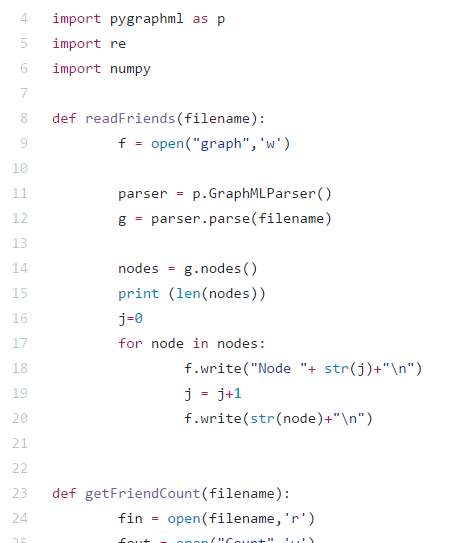
\includegraphics[height=12 cm]{p1code.png}
  \caption{``p1.py" is the Python script that gathers all the twitter information used in the visualization}
\end{figure}
\newpage

All the data for the nodes and links was saved in csv format and then converted to JSON using an online tool (http://www.csvjson.com/csv2json). This was done because it extremely convenient to create a force graph using input from a JSON file. With a great deal of help from Michael Bostock's tutorials on force graphs. As will be seen upon inspection, the main ``source" in the graph is OKMotovlog, whose node was intentionally resized and colored red, to distinguish him from his followers (as if the fact that everyone is connected to him and he is smack in the midlle wasn't enough). The size of the nodes for his followers is determined by the number of followers they have. This was not done using scales (I know it was the perfect opportunity to implement a scale function, but this was done really last minute). Instead, any user with more than 10000 followers had a radius of 30, above 1000 a radius of 20 and bellow 100 a radius of 10. Finally, when we mouseover a node we see the name of the user (not the screen name) and the number of followers they have.

The link to the Github hosted webpage is below:

https://rawgit.com/mmicr001/cs532-s17/master/assignments/assignment6/hw6.html

\begin{figure}[H]
 \centering
 	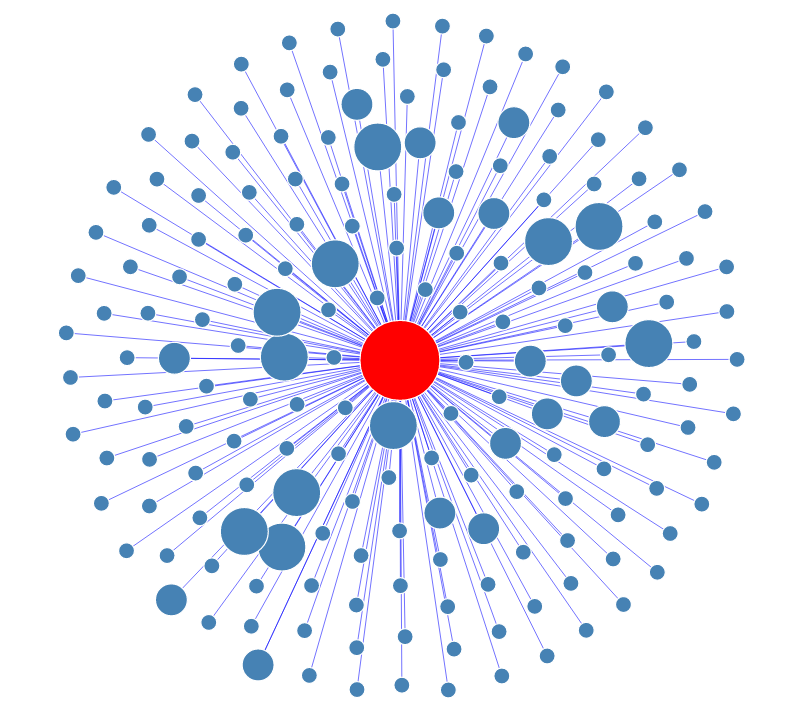
\includegraphics[height=12 cm]{graph.png}
  \caption{Sample output of visualization of OKMotovlog's twitter followers}
\end{figure}

%----------------------------------------------------------------------------------------
\end{document}
